% !Mode:: "TeX:UTF-8"
%!TEX program  = xelatex

\documentclass[bwprint]{cumcmthesis} 

\title{高温工作温度分布模型}
\tihao{A}
\baominghao{201809002232}
\schoolname{上海交通大学}
\membera{钱文涛}
\memberb{盛志耀}
\memberc{王思极}
\supervisor{尚建辉老师}
\yearinput{2018}
\monthinput{9}
\dayinput{14}
\begin{document}
 \maketitle
 \begin{abstract}
    \indent 人们在进行高温作业时需要穿着专业的高温工作服以防危险。通常的高温工作服由三层织物材料构成,本文将研究高温工作服的隔层材料的导热性质,建立数学模型模拟来确定假人皮肤外侧的温度变化情况。\\
    \indent 针对问题一,首先建立系统的热传导方程,系统包括:人体、高温工作服以及外界热源。再考虑到人体表面接触高温工作服,高温工作服同时与外界热源接触,所以不妨将我们的方程简化成为一维热传导方程。\\
    \indent 在建立完一维热传导方程之后,结合已知的边界条件,就可以通过求解微分方程得到系统的温度分布。再将已经求解得到的温度分布与“附件2. 假人皮肤外侧的测量温度”进行比对,如果对比结果直接满足,那可以继续进行问题二、三的求解;反之,则需要对建立的模型进行修正。\\
    \indent 最后经过对比,发现数据的拟合程度确实存在一定的出入,故考虑进行修正。修正一:在工作服表面和75度热源之间有一层薄空气层,记作V层;修正二:人体内环境和工作服之间存在人体组织,记作0层。\\
    \indent 修正之后,再度求解微分方程。最终发现此时的修正结果与附件所给数据符合得很好。\\
    \indent 针对问题二,结合已经求解得到的温度分布模型,修改初始条件为:环境温度为$65^{\circ}C$、IV层的厚度为$5.5mm$,确定出合适的$\uppercase\expandafter{\romannumeral2}$层厚度,使得确保工作60分钟时,假人皮肤外侧温度不超过$47^{\circ}C$,且超过$44^{\circ}C$的时间不超过5分钟。\\
    \indent 针对问题三,结合已经求解得到的温度分布模型,修改初始条件为:环境温度为$80^{\circ}C$,确定出合适的$\uppercase\expandafter{\romannumeral2}$层和$\uppercase\expandafter{\romannumeral4}$层厚度,使得确保工作60分钟时,假人皮肤外侧温度不超过$47^{\circ}C$,且超过$44^{\circ}C$的时间不超过5分钟。\\
    \indent 最后再总体考虑所以材料的参数进行微修正,并做一定的回归分析,控制模型的误差。
\keywords{热传导方程 \quad 温度分布 \quad 误差分析 }
\end{abstract}

\section{问题的提出}
    \indent 实际生活中从事高温环境工作的人员需要穿着专业的高温工作服以防被烧伤。那么根据现有材料的相关参数模拟得出合适的服装设计就十分的重要。另外,热传导方程是一个我们熟知的偏微分方程,它具体描述了一个区域内的温度如何随时间变化。\\

\section{问题重述}
    \indent 现根据附件所提供的专用服装材料的参数值以及假人皮肤外侧的测量温度数据,建立数学模型,解决以下问题:
    \begin{enumerate}
        \item 利用附件problem1.xlsx中的相关材料参数对附件中的家人皮肤测量温度进行模拟,建立模型,计算温度分布,并生成温度分布文件。
        \item 利用在问题一中提出的模型,当环境温度为$65^{\circ}C$、IV层的厚度为$5.5mm$时,确定II层的最优厚度,确保工作60分钟时,假人皮肤外侧温度不超过$47^{\circ}C$,且超过$44^{\circ}C$的时间不超过5分钟。
        \item 利用在问题一种提出的模型,当环境温度为$80^{\circ}C$时,确定$\uppercase\expandafter{\romannumeral2}$层和$\uppercase\expandafter{\romannumeral4}$层的最优厚度,确保工作30分钟时,假人皮肤外侧温度不超过$47^{\circ}C$,且超过$44^{\circ}C$的时间不超过5分钟。
        
    \end{enumerate}

    \section{模型的假设}
    \begin{itemize}
    \item 从一维情况考虑。
    \item 不考虑热辐射和对流。
    \item 假设$75$度是一个稳定热源的温度,它和外层织物存在一个空气层,那一层的初始温度是$75$度,充当了衣物和75度热源之间的缓冲层。
    \item 人的皮肤和内部温度存在一层组织充当热传导材料。
    \item 人体组织和所有衣物以及衣物和人体间的空气初始温度都是$37^{\circ}C$。
    \item 所有过程满足热传导方程。
    \end{itemize}

\section{符号说明}
\begin{tabular}{cc}
 \hline
 \makebox[0.4\textwidth][c]{符号}	&  \makebox[0.5\textwidth][c]{意义} \\ \hline
 u      & 温度($^{\circ}$C) \\ \hline
 s	    & 厚度(cm)  \\ \hline
 t	    & 时间(second)  \\ \hline
 $T_{1}$	& 人体内部温度($37^{\circ}$C) \\ \hline
 $T_{2}$	& 理想外部热源温度($75^{\circ}$C) \\ \hline
 k	    &  热扩散率($m^{2}/s$)) \\ \hline
 $\rho$	    & 密度($kg/m^{2}$))  \\ \hline
 C	    & 比热($J/(kg\cdot^{\circ}C)$)  \\ \hline
 $\lambda$	    & 热传导率($W/(m\cdot^{\circ}C)$  \\ \hline
\end{tabular}
\phantom{1} \\
另外,方便起见,我们把衣物和外部热源之间的空气层、$\uppercase\expandafter{\romannumeral4}$层、$\uppercase\expandafter{\romannumeral3}$,$\uppercase\expandafter{\romannumeral2}$层、$\uppercase\expandafter{\romannumeral1}$层、人体组织层分别记作第0层、第1层、第2层、第3层、第4层、第5层。

\newpage
\section{问题分析}
    \subsection{问题一分析}
        \indent 针对问题一,首先建立系统的热传导方程,系统包括:人体、高温工作服以及外界热源。再考虑到人体表面接触高温工作服,高温工作服同时与外界热源接触,大多数接触面的弧度不大,所以不妨将我们的方程简化成为一维热传导方程。\\
        \indent 在建立完一维热传导方程之后,结合已知的边界条件,就可以通过求解微分方程得到系统的温度分布。再将已经求解得到的温度分布与“附件2. 假人皮肤外侧的测量温度”进行比对,如果对比结果直接满足,那可以继续进行问题二、三的求解;反之,则需要对建立的模型进行修正。\\
        \indent 最后经过对比,发现数据的拟合程度确实存在一定的出入,故考虑进行修正。修正一:在工作服表面吸附有一层薄空气层,记作$\uppercase\expandafter{\romannumeral5}$层;修正二:人体内环境和工作服之间存在人体组织,记作0层。\\
        \indent 修正之后,再度求解微分方程。最终发现此时的修正结果与附件所给数据符合得很好。
    \subsection{问题二分析}
        \indent 结合已经求解得到的温度分布模型,修改初始条件为:环境温度为$65^{\circ}C$、IV层的厚度为$5.5mm$,确定出合适的$\uppercase\expandafter{\romannumeral2}$层厚度,使得确保工作60分钟时,假人皮肤外侧温度不超过$47^{\circ}C$,且超过$44^{\circ}C$的时间不超过5分钟。
    \subsection{问题三分析}
        \indent 结合已经求解得到的温度分布模型,修改初始条件为:环境温度为80ºC,确定出合适的$\uppercase\expandafter{\romannumeral2}$层和$\uppercase\expandafter{\romannumeral4}$层的厚度,使得确保工作60分钟时,假人皮肤外侧温度不超过$47^{\circ}C$,且超过$44^{\circ}C$的时间不超过5分钟。

\newpage

\section{模型描述}
    \indent 首先,我们根据热扩散率的公式$k=\frac{\lambda}{C\rho}$可以计算得到各层的热扩散系数$k$,得到下表格:\\
% Table generated by Excel2LaTeX from sheet 'Sheet1'
\begin{table}[htbp]
    \centering
      \begin{tabular}{|c|c|c|c|c|r|}
      \hline
      \multicolumn{6}{|c|}{专用服装材料的参数值} \bigstrut\\
      \hline
      分层   & \multicolumn{1}{p{5em}|}{密度\newline{}($kg/m^{3}$)} & \multicolumn{1}{p{5em}|}{比热\newline{}($J/(kg\cdot^{\circ}C)$)} & \multicolumn{1}{p{5em}|}{热传导率\newline{}($W/(m\cdot^{\circ}C)$)} & \multicolumn{1}{p{5em}|}{厚度\newline{}($mm$)} & \multicolumn{1}{p{5em}|}{热扩散系数($m^{2}/s$)} \bigstrut\\
      \hline
      I层    & 300   & 1377  & 0.082 & 0.6   & $1.985\times10^{-7}$ \bigstrut\\
      \hline
      II层   & 862   & 2100  & 0.37  & 0.6-25 & $2.044\times10^{-7}$ \bigstrut\\
      \hline
      III层  & 74.2  & 1726  & 0.045 & 3.6   & $3.5137\times10^{-7}$ \bigstrut\\
      \hline
      IV层   & 1.18  & 1005  & 0.028 & 0.6-6.4 & $2.3611\times10^{-5}$ \bigstrut\\
      \hline
      \end{tabular}%
      \caption{专用服装材料的参数值表}
    \label{tab:addlabel}%
  \end{table}%

  \indent 根据热传导方程:
  \begin{equation}
      \centering
      \frac{\partial u}{\partial t}=k\frac{\partial^{2}u}{\partial^{2}s}
  \end{equation}
  \indent 我们通过换元,令$s=\sqrt{k}x$,即$x=sk^{-\frac{1}{2}}$,称$x$为等效位移,厚度经过这个换元之后成为等效厚度,得到:
  \begin{equation}
      \centering
      \frac{\partial u}{\partial t}=\frac{\partial^{2}u}{\partial^{2}x}
  \end{equation}
  \indent 把第0、1、2、3、4、5层的等效厚度分别记为$d_0,d_1,d_2,d_3,d_4,d_5$,它们的总等效厚度记为$a$,把第0层的等效厚度和a的比例记作$\alpha$。我们假定人体和所有衣物以及他们中间的空气层的初始温度为37度,而第0层(外部空气)的初始温度为75度,可得初始条件如下:
  \begin{equation}  
    \centering
    u(x,0)=\left\{  
     \begin{array}{lr}  
        T_{1}\quad0<x<\alpha a \\   
        T_{2}\quad\alpha a<x<a 
     \end{array}  
    \right.
\end{equation} 
    \indent 以及边界条件如下:
    \begin{equation}
        \centering
        \left\{  
     \begin{array}{lr}  
        u(0,t)=T_{1} \\   
        u(a,t)=T_{2}
     \end{array}  
    \right.
\end{equation}
  
    \indent 根据微分方程理论,方程$(1)$的通解具有如下形式:
    \begin{equation}
        \centering
        \left\{  
     \begin{array}{lr}  
        (c_{1}\sin(\omega x)+c_{2}\cos(\omega x))e^{-\omega^{2}t} \\   
        d_{1}x+d_{2} \\
        (c_{1}e^{\omega x}+c_{2}e^{-\omega x})e^{\omega^{2}t}
     \end{array}  
    \right.
    \end{equation}
    
    \indent 根据边界条件,选择$u(x,t)$的形式为:
    \begin{equation}
        u(x,t)=\frac{T_{2}-T_{1}}{a}x+T_{1}+\sum_{n=1}^{\infty}A_{n}\sin(\frac{n\pi}{a}x)e^{-\frac{n^{2}\pi^{2}}{a^{2}}t}
    \end{equation}
    \indent  代入边界条件,边界条件显然成立,对于初始条件,我们有:
    \begin{equation}
        \sum_{n=1}^{\infty}A_{n}\sin(\frac{n\pi}{a}x)e^{-\frac{n^{2}\pi^{2}}{a^{2}}t} = \left\{\begin{array}{cc}
        \frac{T_1-T_2}{a} x & (0\leq x \leq \alpha a)\\
        (T_2-T_1)(1-\frac{x}{a})& (\alpha a \leq x \leq a)
        \end{array} \right.
    \end{equation}
    \begin{equation}
        \centering
        \int_{0}^{a}\sin(\frac{n\pi}{a}x)(\sum_{n=1}^{\infty}A_{n}\sin(\frac{n\pi}{a}x))dx=\frac{a}{2}A_{n}
    \end{equation}
    \begin{equation}
        \frac{a}{2}A_{n}=\int_{0}^{\alpha a} \sin(\frac{n\pi}{a}x)\frac{T_1-T_2}{a} x dx + \int_{\alpha a}^{a}\sin(\frac{n\pi}{a}x)(T_2-T_1)(1-\frac{x}{a}) dx
    \end{equation}
    \indent 通过积分运算,我们可以计算出$A_{n}$的值:
    \begin{equation}
        A_n=2\frac{T_2-T_1}{n\pi} \cos(n\pi \alpha)
    \end{equation}
    \indent 而温度分布为函数为:
    \begin{equation}
        u(x,t)=\frac{T_{2}-T_{1}}{a}x+T_{1}+\sum_{n=1}^{\infty}2\frac{T_2-T_1}{n\pi} \cos(n\pi \alpha)\sin(\frac{n\pi}{a}x)e^{-\frac{n^{2}\pi^{2}}{a^{2}}t}
    \end{equation}
    \indent 可以看出,随着时间增加,温度分布将趋于一条直线,这很符合我们常理。
    \indent 接下来,我们开始利用python程序来验证我们的想法。利用人工智能相关模块pytorch并秉承并行化计算的思想,我们设计了高效的计算$u(x,t)$的函数,并且只对无穷级数的前1000项和10000项作求和,发现这两种方式下得到的误差结果没有任何区别,故取前1000项是一个合理的近似。\\

    \indent 我们不知道第0层(外部空气))和第5层(人体组织)的等效厚度,但是我们从附件2中得知,在75度的外部环境中,皮肤表面的平衡温度为48.0799度。我们先计算了第1、2、3、4层的总等效厚度$d_1+d_2+d_3+d_4$,为$21.72022 s^{1/2}$,根据平衡状态下温度分布为一条直线$(T = \frac{75-47}{a}x+37)$的性质,得到以下的方程:
    \begin{equation}
        d_5 = \alpha a - 21.72022
    \end{equation}
    \begin{equation}
        \frac{75-37}{a}d_5 + 37 = 48.0799    
    \end{equation}
    \indent $d_0$,$a$可以根据$\alpha$确定。同时$d_5$等于$(1-\alpha)a$,也可以确定。所以我们把$\alpha$作为一个自变量来计算温度分布,和$x=d_0$(皮肤表面)处的温度变化情况。经过一段时间的调整,我们找到了一个$\alpha$最优解:
    \begin{equation}
        \centering
        \left\{  
     \begin{array}{lr}  
        \alpha=0.75 \\   
        a=47.380508849 \\
        d_0=13.815158896
     \end{array}  
    \right.
    \end{equation}
    \indent  我们计算了这种情况下,在$x=d_0$,也就是皮肤表面的温度时间曲线,所有时刻下我们的函数的预测值和温度实际值的误差的绝对值的平均值,为0.0042度(这更有可能使由于测量温度时的精度限制导致的),这个函数很好地模拟了温度的分布。下面是我们的函数预测值和实际温度的对比图。
    \begin{flushleft}
        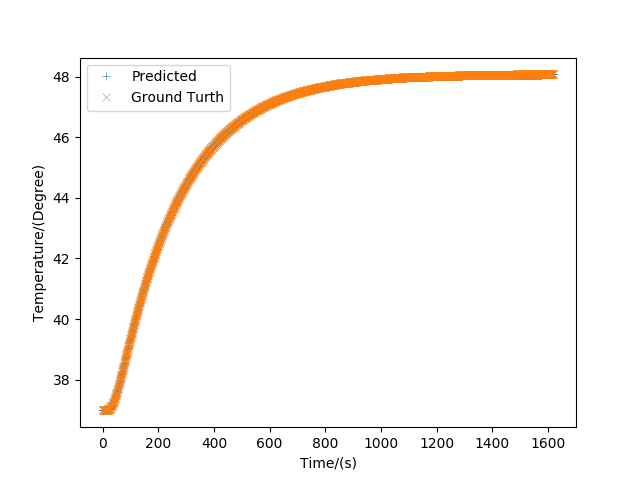
\includegraphics[scale = 1]{Problem1.png}
    \end{flushleft}
    \indent 这种情况下难以看到它们的差别,接下来是放大后的的对比图:
    \begin{flushleft}
        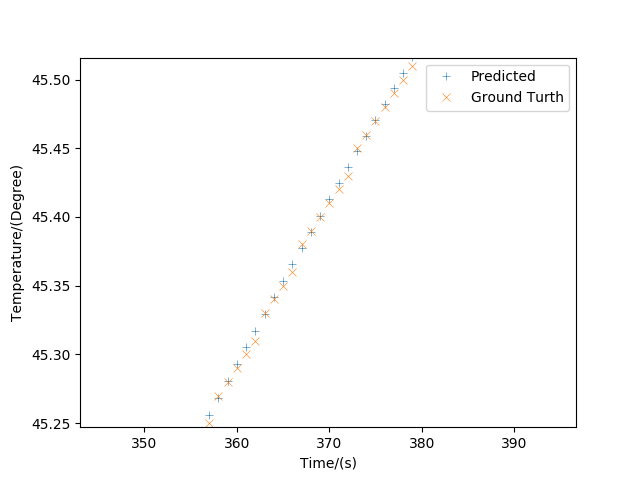
\includegraphics[scale=1]{Problem11.png}
    \end{flushleft}
    \indent 我们的模型非常成功地预测了人体表面温度随时间的变化,所以我们可以很有自信地利用它来解决3个问题。

\section{问题一}
\indent 模型的提出和推导已经完成,这里解释我们计算温度随时间和位移变化的关系的过程。我们把第1、2、3、4层的所占的实际厚度(15.2mm)分成500等分,把它们转化等效位移$x$,然后根据我们解出的温度随时间、等效位移的变化关系$u(x,t)$计算每一个位置和时间对应的温度,并生成了excel文件。它的第一行代表了500个实际位移位置(以mm为单位)的值,第一列则是时间轴,每个位置和时间的对应一个温度。这是根据我们计算的温度随时间位移分布的三维图(由于在时间超过1600秒后,温度变化已经不明显,所以省去这部分):
\begin{flushleft}
    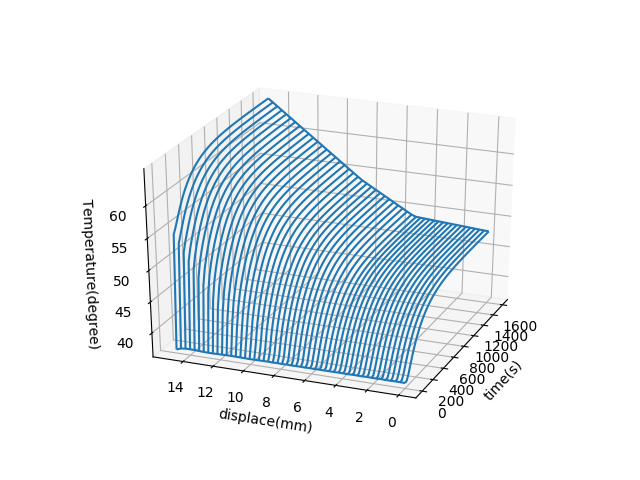
\includegraphics[scale=1]{Problem_12.png}
\end{flushleft}

\section{问题二}
\indent 问题重述:当环境温度为65ºC、IV层的厚度为5.5 mm时,确定II层的最优厚度,确保工作60分钟时,假人皮肤外侧温度不超过47ºC,且超过44ºC的时间不超过5分钟。\\
\indent 为了提高工作服的舒适度,应该让工作服尽量薄一些,而且同时还要满足隔热的要求,所以我们寻求这么一个最优解,既可以达到隔热要求,又能使衣物尽量薄。在第4层厚度已经确定的前提下,我们利用建立的模型,计算不同第2层厚度对应的温度时间变化关系。这里主要改变的是我们的模型中$a$和$\alpha$变量,计算的仍然是皮肤表面的温度变化,$u(d_5,t)$,只要根据不同的第二层厚度,$d_2$修改它们即可。计算公式如下:
\begin{equation}
    a = \sum_{i=0}^5 d_i
\end{equation}
\begin{equation}
    \alpha = 1-d_5/a
\end{equation}
\indent 经过实验,我们找到了一个合适的$d_2$的值,$d_2=9.51529$mm,在这种情况下,皮肤的最高温度为44.0001度,超过44度的时间是296s。这是它的温度时间曲线(其中蓝色的线标志着温度超过44度):
\begin{flushleft}
    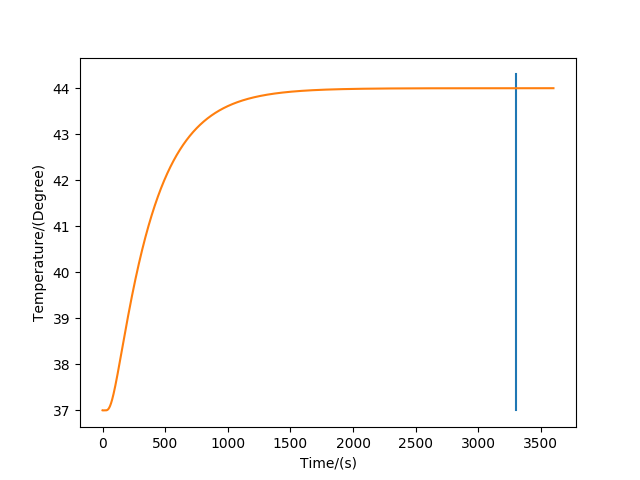
\includegraphics[scale=1]{Problem2.png}
\end{flushleft}

\section{问题三}

\indent 问题重述:当环境温度为80时,确定II层和IV层的最优厚度,确保工作30分钟时,假人皮肤外侧温度不超过47ºC,且超过44ºC的时间不超过5分钟。\\
\indent 这个问题与问题二没有本质上的差别,我们依旧通过调整$d_2$的方式来解决。这里我们仍然保持$d_4$不变,为5.5mm,因为这个厚度处于正常的范围,且没有什么用来衡量空气层对人体带来影响的指标。最终得到的解为,$d_2=18.366$mm。这种情况下,最高温度为44.3855度,超过44度的时间为300秒。以下使这种情况对应的时间温度变化曲线:\newpage
\begin{equation}
    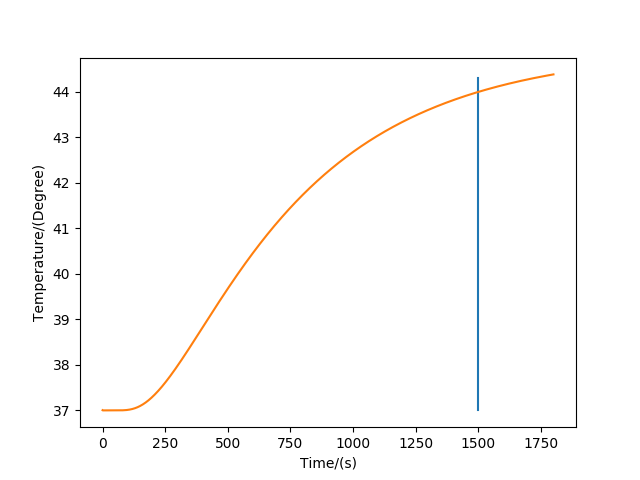
\includegraphics[scale=1]{Problem3}
\end{equation}

\section{python代码}
语言:\\
python2.7
模块:\\
torch\\ 
numpy\\
matplotlib\\
xlrd\\
xlsxwriter\\
\subsection{}

    

    
    
     








\end{document} 